We will first provide some basic definitions about particles and paths, which will lay the groundwork for thinking about fastest paths. First we will define what we mean by a particle and a path.

\begin{definition}
  A path $\gamma(t): [T_0(\gamma), T_f(\gamma)] \to \mathrm{R}^2$ is a function which maps a time $t \in [T_0(\gamma), T_f(\gamma)]$ to a position $\bvec{X} \in \mathrm{R}^2$.
\end{definition}

\begin{definition}
  A particle $p$ is an object in space with zero volume. If a particle is traveling along a path, $\gamma(t)$, then we define a position, $\bvec{X}(t) \coloneqq \gamma(t)$, a velocity, $\bvec{v}(t) \coloneqq \frac{d\gamma(t)}{dt}$, and an acceleration, $\bvec{a}(t) \coloneqq \frac{d^2\gamma(t)}{dt^2}$, for the particle, for all $t \in [T_0(\gamma), T_f(\gamma)]$.

  A particle is restricted if there are conditions on its position and the time derivatives of its position. Given a particle, a valid path is a path that the particle can travel along without violating its restrictions.
\end{definition}

Now we will make our problem statement more rigorous, by defining what a fastest path is.

\begin{definition}
  Let $p$ be a particle with initial position $X_0$, a fastest path $\hat{\gamma}(t)$ to $\bvec{X_f}$, is a valid path such that $T_f(\hat{\gamma}) \leq T_f(\gamma)$ for all valid paths $\gamma(t)$ to $\bvec{X_f}$.
\end{definition}

Finally, we need to define some terms for a particle's motion which will be needed later on to describe restrictions on a particle's motion.

\begin{definition}
  The centripetal acceleration $\bvec{a_c}(t)$ of a particle, $p$, is the component of its acceleration in the direction perpendicular to its direction of motion.
\end{definition}

\begin{definition}
  The tangential acceleration $a_t(t)$ of a particle is the component of the acceleration of the particle in its direction of motion.

  \begin{equation}
    a_t(t) \coloneqq \frac{dv(t)}{dt}
  \end{equation}
\end{definition}
% -----------------------------------------------------------------------------

\subsection{Particle Motion in Polar Coordinates}

Before we introduce the equations governing a particle's motion in $\R^2$, we must first define a coordinate system to describe its motion. Unless otherwise specified, the motion of particles in this paper will be described in a modified polar coordinate system that contain an extra parameter $\theta$, that is shown in Figure \ref{fig:polar-param}. We will refer to this system as the \textit{B centered particle coordinate system}.

\begin{figure}[H]
    \begin{center}
      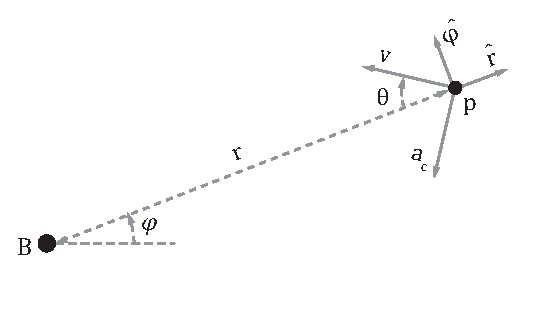
\includegraphics[width=4in,height=3in,keepaspectratio]{polar_param.eps}
    \end{center}
  \vspace{-.2in} % corrects bad spacing
  \caption{A particle moving in a B centered particle coordinate system.\label{fig:polar-param}}
  \end{figure}

The sign of $a_c(t)$ is defined to be the sign of the projection of $\bhat{a_c}(t)$ onto $-\bhat{r}(t)$; in other words, it is positive when pointing towards B. $\theta(t), \phi(t) \in [-\pi, \pi]$, and from now on, we will only use $\abs{\theta(t)}$ and $\abs{\phi(t)}$, since there is a symmetry in the system about $\bhat{r}$. 

\begin{lemma}
The time derivative of $\abs{\theta(t)}$ is given by

\begin{equation}\label{eq:theta-deriv}
\frac{d\abs{\theta(t)}}{dt} = \frac{d\abs{\phi(t)}}{dt} + \frac{a_c(t)}{v(t)}
\end{equation}

\end{lemma}

\begin{proof}

$\theta(t)$ is composed of $\phi(t)$ plus the angle between $\bhat{v}(t)$ and the horizontal, which we can temporarily call $\beta(t)$. $\phi(t)$ is the component of $\theta(t)$ in the polar coordinate system, and changes as the point moves with respect to the point B. $\beta(t)$ can be thought of as the component of $\theta(t)$ in the Cartesian coordinate system, and it only changes when $a_c(t)$ is nonzero. 

Differentiating, we get

\[
\frac{d\abs{\theta(t)}}{dt} = \frac{d\abs{\phi(t)}}{dt} + \frac{d\beta(t)}{dt}
\]

To find $\frac{d\beta(t)}{dt}$, we can look at a point, $p$, subject to nonzero centripetal acceleration, and zero tangential acceleration. The change in $\bvec{v(t)}$ over an infinitesimal time, $dt$, is shown below (the two vectors, $\bvec{v(t)}$ and $\paren{\bvec{v(t)}+\bvec{dv(t)}}$, are superimposed). 

\begin{figure}[H]
    \begin{center}
      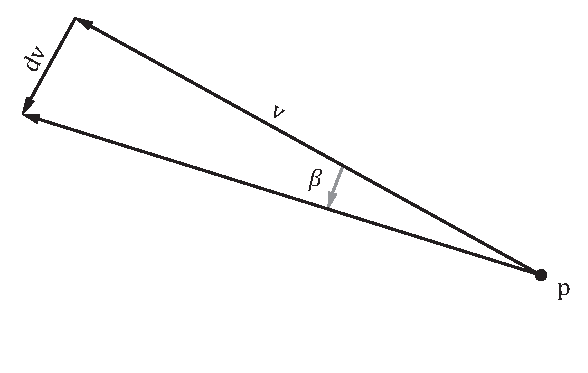
\includegraphics[width=3.5in,height=2.5in,keepaspectratio]{theta_deriv.eps}
    \end{center}
  \vspace{-.2in} % corrects bad spacing
  \caption{}
\end{figure}

$a_c(t)$ is defined to be the component of acceleration perpendicular to the direction of motion, so

\[
\frac{dv(t)}{dt} = a_c(t)
\]

Since $dv(t) = -d\beta(t) v(t)$, then

\[
\frac{d\beta(t)}{dt} = -\frac{a_c(t)}{v(t)}
\]

The proof of the lemma in the case where $a_t(t)$ is nonzero is nearly identical, since the component of $\bvec{dv}(t)$ in the direction $\bhat{v}(t)$ is negligible compared to $v(t)$.

\end{proof}

Returning again to Figure \ref{fig:polar-param}, the following equations can be derived

\begin{align}
  \frac{dr(t)}{dt}& = -v(t) \, \cos\paren{\abs{\theta(t)}}\label{eq:r-diff}\\
  \frac{d\abs{\phi(t)}}{dt}& = \frac{v(t)}{r(t)} \, \sin\paren{\abs{\theta(t)}}\label{eq:phi-diff}\\
  \frac{d\abs{\theta(t)}}{dt}& = \frac{d\abs{\phi(t)}}{dt} - \frac{a_c(t)}{v(t)}\\
  &= \frac{v(t)}{r(t)} \, \sin\paren{\abs{\theta(t)}} - \frac{a_c(t)}{v(t)}\label{eq:theta-diff}\\
  \intertext{Applying the chain rule to (\ref{eq:r-diff})}
  \frac{d}{dt} \frac{dr(t)}{dt}& = -\frac{dv(t)}{dt} \cos\paren{\abs{\theta(t)}} + v(t) \sin\paren{\abs{\theta(t)}} \frac{d\abs{\theta(t)}}{dt}\\
  &\begin{aligned}
    = -a_t(t) \cos\paren{\abs{\theta(t)}} &+ \frac{v(t)^2}{r(t)} \sin^2\paren{\abs{\theta(t)}}\\
    &\qquad - \sin\paren{\abs{\theta(t)}} a_c(t) \label{eq:r-diff-2}
  \end{aligned}
\end{align}
